% exercise sheet with header on every page for math or close subjects
\documentclass[12pt]{article}
\usepackage[utf8]{inputenc}
\usepackage{latexsym}
\usepackage{multicol}
\usepackage{fancyhdr}
\usepackage{amsfonts}
\usepackage{amsmath}
\usepackage{amssymb}
\usepackage{enumerate}
\usepackage{listings}
\usepackage{graphicx}
\usepackage{amssymb}

% Shortcuts for bb, frak and cal letters
\newcommand{\E}{\mathbb{E}}
\newcommand{\V}{\mathbb{V}}
\renewcommand{\P}{\mathbb{P}}
\newcommand{\N}{\mathbb{N}}
\newcommand{\R}{\mathbb{R}}
\newcommand{\C}{\mathbb{C}}
\newcommand{\Z}{\mathbb{Z}}
\newcommand{\Pfrak}{\mathfrak{P}}
\newcommand{\Pfrac}{\mathfrak{P}}
\newcommand{\Bfrac}{\mathfrak{P}}
\newcommand{\Bfrak}{\mathfrak{B}}
\newcommand{\Fcal}{\mathcal{F}}
\newcommand{\Ycal}{\mathcal{Y}}
\newcommand{\Bcal}{\mathcal{B}}
\newcommand{\Acal}{\mathcal{A}}

% formating
\topmargin -3.5cm
\textheight 22cm
\textwidth 16.0 cm
\oddsidemargin -0.1cm

% Fancy Header on every Page
\pagestyle{fancy}
\lhead{\textbf{Embedded Systems Milestone 6}}
\rhead{Rafael Dewes (2548365) \\ Kevin M\"uller (2550062) \\ Daniel Schäfer (2549458)\\ }
\renewcommand{\headrulewidth}{1.2pt}
\setlength{\headheight}{110pt}

\begin{document}
\pagenumbering{gobble}
\lstset{language=C++}

\section*{Test Series}
\subsection*{Line Sensor Readings}
We tested the line sensors in different lighting environments and for multiple line colours.
Using the sensor in the center, we calibrated the robot for a bright environment, moderate lighting and dark environment each, then let it detect lines of different color.

\begin{tabular}{ | l || r | r | r | r | r | }
\hline
Lighting & Readings for & & & & \\
Conditions & White ground & Black line & Grey line & Blue line & Red line \\ \hline
Bright & 0 & 1000 & 158 & 92 & 56\\ \hline
Medium & 0 & 1000 & 186 & 100 & 64\\ \hline
Dark & 0 & 940 & 131 & 66 & 33\\
\hline
\end{tabular}

\begin{center}

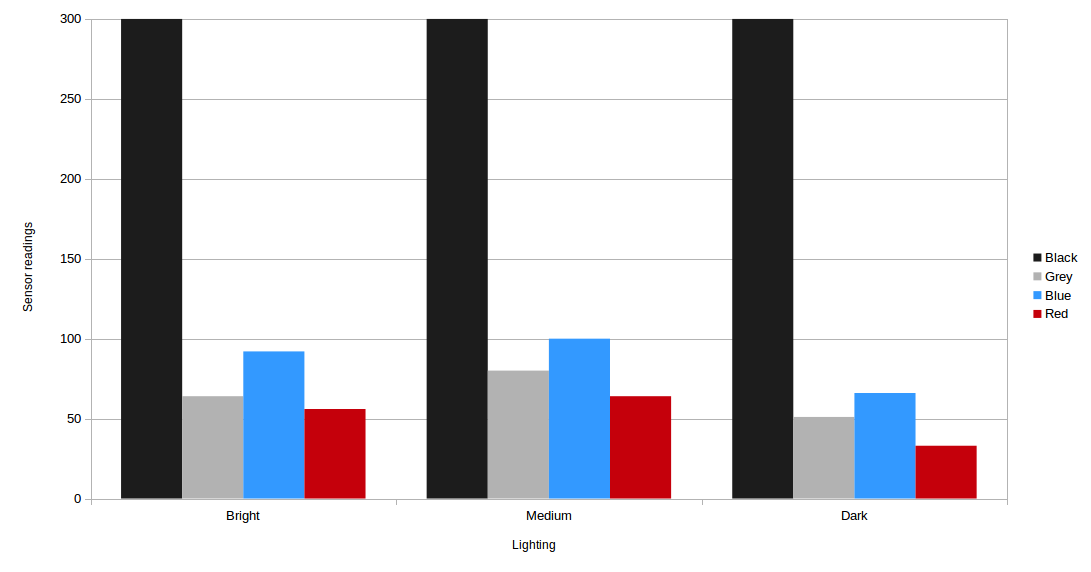
\includegraphics[width = 0.8\textwidth]{images/chart_brightness.png}


\textit{(The y axis is capped at 300 for readibility reasons.)}

\end{center}

\subsection*{Velocity vs. Line Count}
The following table contains our results from testing the accuracy of the line sensors for different velocities. We let the robot drive in the arena at different speeds and instructed to stop after a certain number of lines counted. This worked perfectly for any speed.


\begin{tabular}{ | c || r | r | r | }
\hline
Velocity & Lines Crossed & Lines Counted & $\Delta$ Lines \\
 & & &  \\ \hline
Slow & 3 & 3 & $\pm 0$  \\ \hline
(50) & 10 & 10 & $\pm 0$  \\ \hline
Medium & 3 & 3 & $\pm 0$  \\ \hline
(100)  & 10 & 10 & $\pm 0$  \\ \hline
Fast & 3 & 3 & $\pm 0$ \\ \hline
(200) & 10 & 10 & $\pm 0$ \\ \hline
Max & 3 & 3 & $\pm 0$  \\ \hline
(400) & 10 & 10 & $\pm 0$  \\ \hline
\end{tabular}

\subsection*{Velocity vs. Referee Updates}
Accuracy of the position updates sent by the referee for different velocities.
To test this the robot drives 100cm through the arena at a different speed each; 
we monitor the referee interface and send position updates every second.


\begin{tabular}{ | c || r | r | r | }
\hline
Velocity & Number of & Estimated Distance & Update Delay \\
  & unique Updates & per Update &  \\ \hline
Slow & $>$50 & ~1cm & 0.5s  \\ 
(50) &  & &  \\ \hline
Medium & 31 & 3cm & 0.5s \\ 
(100) &  &  &  \\ \hline
Fast & 8 & 15cm & 0.5s \\ 
(200) &  &  &  \\ \hline
Max & 2 & 100cm & 4s \\ 
(400) &  &  &  \\ \hline
\end{tabular}

The results show that the referee is at least half a second delayed, and we found that for speeds above 300 it cannot track the robots sufficiently. Below that we just cover more distance between the referees updates for faster velocities, which makes the position updates less accurate.

\section*{Testing Against a Model}

\subsection*{Timed Automaton}
\begin{center}


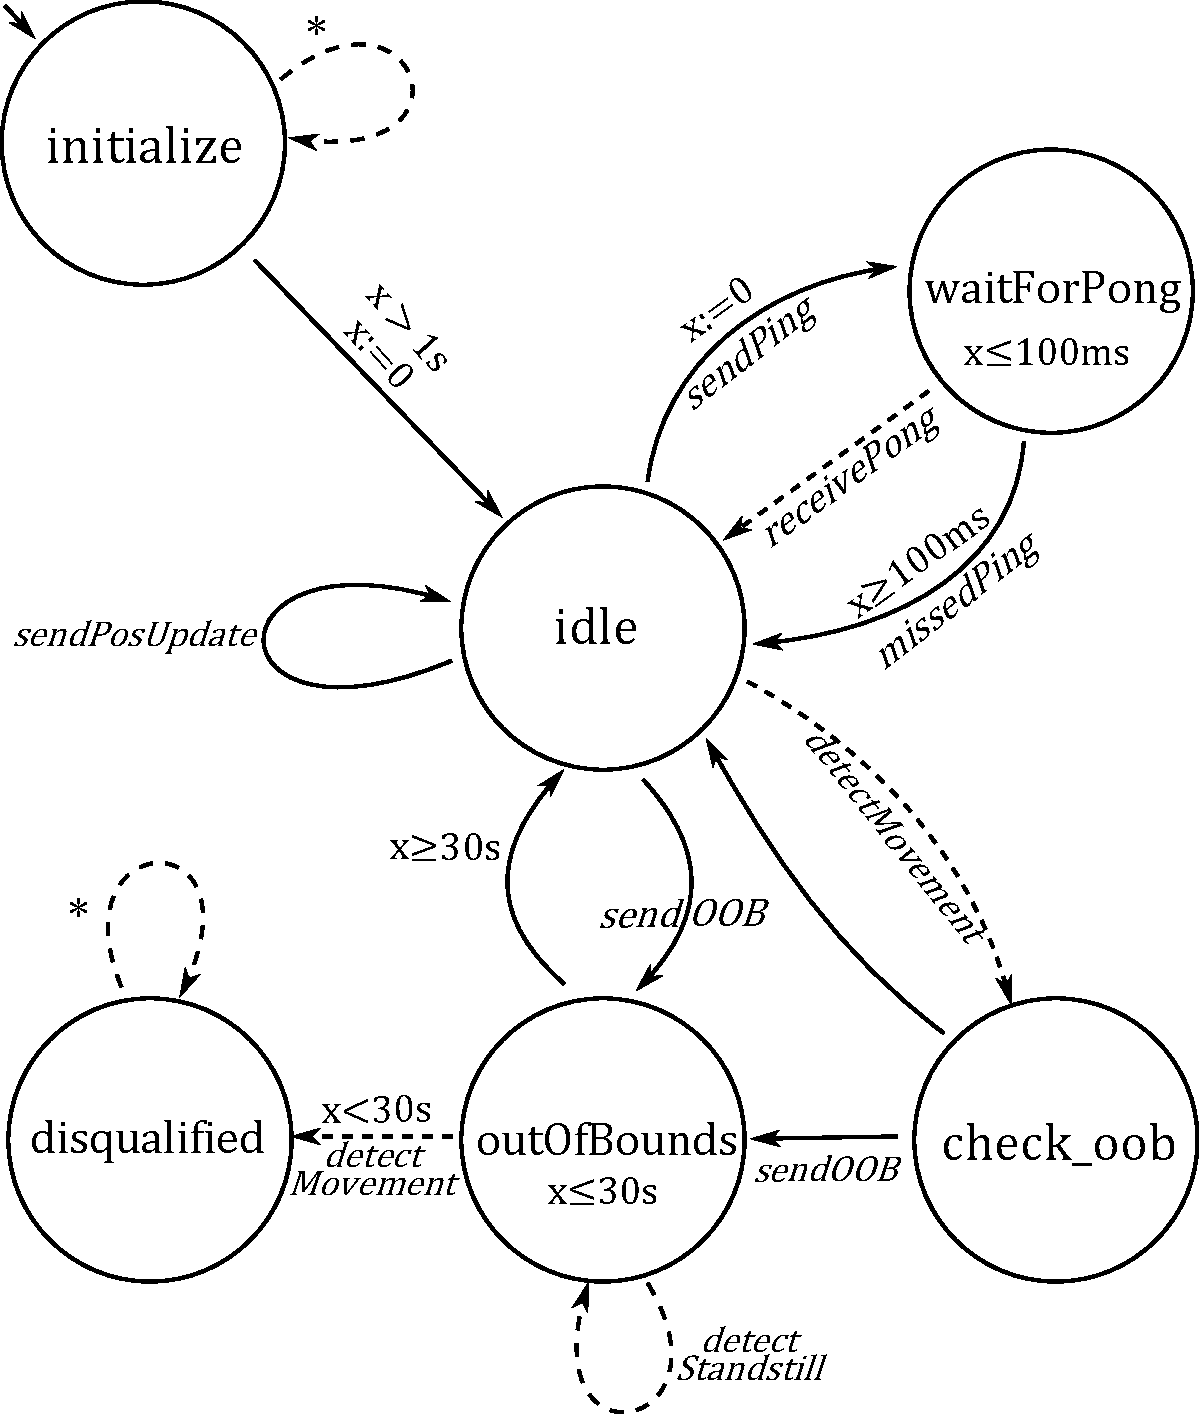
\includegraphics[width = 0.75\textwidth]{images/ref_ta.pdf}

Timed automaton representing the referee.

\end{center}

\subsection*{Testing Runs}
We have one run to test the robot's reaction to ping:
\[ \tau \rightarrow (sendPing \rightarrow \tau \rightarrow receivePong)^{*}  \] 

\flushleft
The second run secures that the robot reacts correctly to an Out-of-bounds message:
\[ \tau \rightarrow sendPosUpdate\rightarrow sendOOB \rightarrow (detectStandstill | \tau )^{*} \rightarrow penaltyOver \rightarrow \dots \]

\subsection*{Implementation and Changes}
To model the nondeterminism we introduced a random variable into the simulation. Pings are sent at irregular intervals, and wait times after every transition are randomized.
\end{document}

